\documentclass{beamer}

\usepackage{amsmath}
\usepackage{amssymb}
\usepackage{tikz}
\usepackage{pgfplots}

\title{Symmetric Matrices}
\subtitle{\(A = A^T\)}
\author{Ahmed Mohammed}
\institute{Georgia Institute of Technology}
\date{PLUS Session, Summer 2023}

\usetheme{Antibes}
\usefonttheme{serif}

\renewcommand{\vec}[1]{\mathbf{#1}}

\AtBeginSection[]
{
    \begin{frame}
        \frametitle{Table of Contents}
        \tableofcontents[currentsection]
    \end{frame}
} % https://statisticaloddsandends.wordpress.com/2019/02/18/beamer-inserting-section-slides-before-each-section/

\begin{document}
	\begin{frame}
		\maketitle
	\end{frame}

	\section{Open Activity}
	\begin{frame}
		\frametitle{Recap}
		\begin{itemize}
			\item<1-> \(A = A^T.\)
			\item<2-> What's special about their eigenvalues?
			\item<3-> What's special about their eigenspaces?
		\end{itemize}
	\end{frame}

	\begin{frame}
		\frametitle{One (Two) Last Special Thing(s)}
		\begin{itemize}
			\item<1-> Every symmetric matrix is \emph{orthogonally} diagonalizable.
				\begin{itemize}[<+(1)->]
					\item \(A = PDP^T.\)
				\end{itemize}
			\item<2-> Note that the columns of \(P\) are \(n\) linearly independent eigenvectors of \(A\) and \(D\) holds its eigenvalues.
			\item<3-> In its expanded form, if \(P = \begin{bmatrix}\vec{u}_1 & \vec{u}_2 & \dots & \vec{u}_n\end{bmatrix}\) and 
					\(D = \begin{bmatrix}\lambda_1 & \dots & 0 \\ \vdots & \ddots & 0 \\ 0 & 0 & \lambda_n \end{bmatrix},\) then what do we get?
		\end{itemize}
	\end{frame}

	\begin{frame}
		\frametitle{The Spectral Decomposition}
		\begin{block}{\textit{Yet Another Decomposition}}
			If \(A \in \mathbb{R}^{n \times n}\) is a symmetric matrix, then it could be decomposed as follows: 
			\[A = \lambda_1 \vec{u}_1\vec{u}_1^T + \lambda_2 \vec{u}_2\vec{u}_2^T + \dots + \lambda_n\vec{u}_n\vec{u}_n^T,\] where 
			\(\vec{u}_1, \dots, \vec{u}_n\) are its \(n\) linearly-independent eigenvectors and \(\lambda_1, \dots, \lambda_n\) are its corresponding 
			eigenvalues.
		\end{block}
		What does this mean geometrically?
	\end{frame}

	\begin{frame}
		\frametitle{Geomtric Intuition}
		\begin{figure}[!h]
			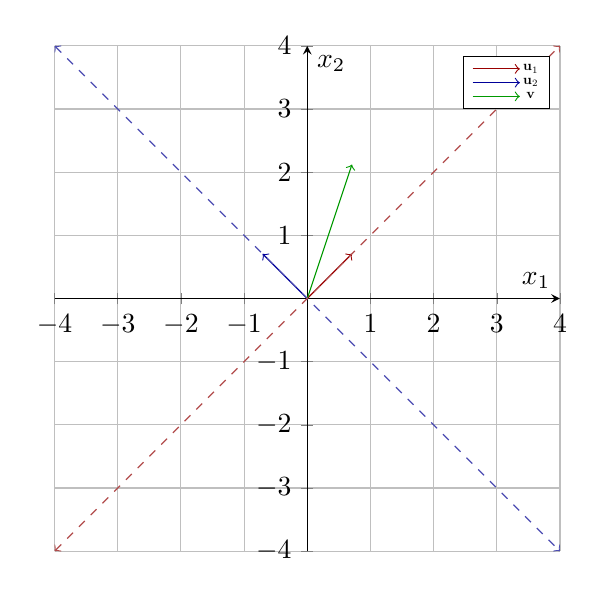
\begin{tikzpicture}
				\begin{axis}
					[axis lines=middle, height=8cm, width=8cm, xmin=-4, xmax=4, ymax=4, ymin=-4,
					 xlabel=\(x_1\), ylabel=\(x_2\), grid=both, xtick distance = 1, ytick distance = 1,
					legend style={nodes={scale=0.5, transform shape}}] % Thanks tex.stackexchange

					\addplot[->, color=red!60!black] coordinates {(0, 0) (0.7071, 0.7071)};
					\addlegendentry{\(\vec{u}_1\)}
					
					\addplot[->, color=blue!60!black] coordinates {(0, 0) (-0.7071, 0.7071)};
					\addlegendentry{{\(\vec{u}_2\)}}

					\addplot[->, color=green!60!black] coordinates {(0, 0) (0.7071, 2.121)};
					\addlegendentry{{\(\vec{v}\)}}


					\addplot[<->, domain=-4:4, color=blue!40!gray, dashed] {-x};
					\addplot[<->, domain=-4:4, color=red!40!gray, dashed] {x};
				\end{axis}
			\end{tikzpicture}
		\end{figure}
	\end{frame}

	\begin{frame}
		\frametitle{Geomtric Intuition}
		\begin{figure}[!h]
			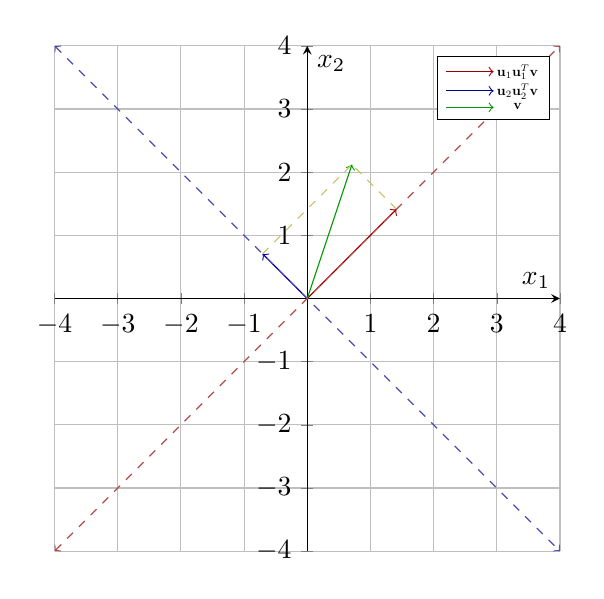
\begin{tikzpicture}
				\begin{axis}
					[axis lines=middle, height=8cm, width=8cm, xmin=-4, xmax=4, ymax=4, ymin=-4,
					 xlabel=\(x_1\), ylabel=\(x_2\), grid=both, xtick distance = 1, ytick distance = 1,
					legend style={nodes={scale=0.5, transform shape}}] % Thanks tex.stackexchange

					\addplot[->, color=red!60!black] coordinates {(0, 0) (1.414, 1.414)};
					\addlegendentry{\(\vec{u}_1\vec{u}_1^T\vec{v}\)}
					
					\addplot[->, color=blue!60!black] coordinates {(0, 0) (-0.7071, 0.7071)};
					\addlegendentry{{\(\vec{u}_2\vec{u}_2^T\vec{v}\)}}

					\addplot[->, color=green!60!black] coordinates {(0, 0) (0.7071, 2.121)};
					\addlegendentry{{\(\vec{v}\)}}


					\addplot[dashed, color=yellow!50!gray] coordinates {(-0.7071, 0.7071) (0.7071, 2.121)};
					\addplot[dashed, color=yellow!50!gray] coordinates {(1.414, 1.414) (0.7071, 2.121)};

					\addplot[<->, domain=-4:4, color=blue!40!gray, dashed] {-x};
					\addplot[<->, domain=-4:4, color=red!40!gray, dashed] {x};
				\end{axis}
			\end{tikzpicture}
		\end{figure}
	\end{frame}

	\begin{frame}
		\frametitle{Geomtric Intuition}
		\begin{figure}[!h]
			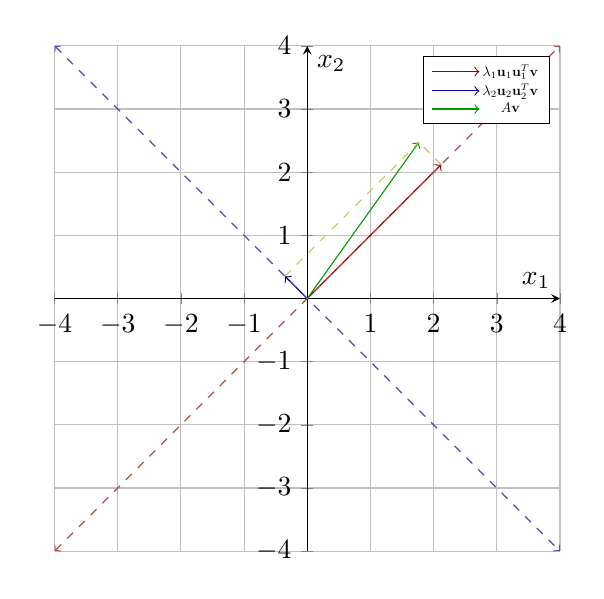
\begin{tikzpicture}
				\begin{axis}
					[axis lines=middle, height=8cm, width=8cm, xmin=-4, xmax=4, ymax=4, ymin=-4,
					 xlabel=\(x_1\), ylabel=\(x_2\), grid=both, xtick distance = 1, ytick distance = 1,
					legend style={nodes={scale=0.5, transform shape}}] % Thanks tex.stackexchange

					\addplot[->, color=red!60!black] coordinates {(0, 0) (2.121, 2.121)};
					\addlegendentry{\(\lambda_1\vec{u}_1\vec{u}_1^T\vec{v}\)}
					
					\addplot[->, color=blue!60!black] coordinates {(0, 0) (-0.3535, 0.3535)};
					\addlegendentry{{\(\lambda_2\vec{u}_2\vec{u}_2^T\vec{v}\)}}

					\addplot[->, color=green!60!black] coordinates {(0, 0) (1.7675, 2.4745)};
					\addlegendentry{{\(A\vec{v}\)}}


					\addplot[dashed, color=yellow!50!gray] coordinates {(-0.3535, 0.3535) (1.7675, 2.4745)};
					\addplot[dashed, color=yellow!50!gray] coordinates {(2.121, 2.121) (1.7675, 2.4745)};

					\addplot[<->, domain=-4:4, color=blue!40!gray, dashed] {-x};
					\addplot[<->, domain=-4:4, color=red!40!gray, dashed] {x};
				\end{axis}
			\end{tikzpicture}
		\end{figure}
	\end{frame}



	\section{Main Activity}
	\begin{frame}
		\frametitle{Exercises}
		\begin{itemize}
			\item<1-> Can \(A\) be symmetric and \(A^2\) be non-symmetric?
			\item<2-> \textit{True, or false.} Every matrix of the form \(A^TA\) has a no negative eigenvalues.
			\item<3-> \textit{True, or false.} If \(\vec{v}_1, \vec{v}_2 \in \mathbb{R}^n\) with \(\vec{v}_1 \ne \vec{v}_2\) are eigenvectors of a 
					symmteric matrix, then \(\vec{v}_1 \cdot \vec{v}_2 = 0.\)
			\item<4-> Every symmetric matrix has \(n\) distinct eigenvalues.
			\item<5-> Find the orthogonal diagonalization of the matrix \(A = \begin{bmatrix}3/2 & 0 & 1/2 \\ 0 & 1 & 0 \\ 1/2 & 0 & 3/2\end{bmatrix}.\)
			\item<6-> \textit{True, or false}. \(Q(\vec{x}) = \|\vec{x}\|^2\) is a quadratic form.
		\end{itemize}
	\end{frame}
	

	\section{Closing Activity}
	\begin{frame}
		There are different types of quadratic forms. \pause
			\begin{itemize}
				\item Positive definite.
					\begin{itemize}
						\item Positive semi-definite.
					\end{itemize}
				\item Negative definite.
					\begin{itemize}
						\item Negative semi-definite.
					\end{itemize}
				\item Indefinite.
			\end{itemize}
		Turns out that the eigenvalues of a symmetric matrix dictate what type of quadratic form we get. \pause

		We also might want to know the maximum (or minimum) value a quadratic form takes when we restrict our input space to unit vectors only.\pause

		Again, eigen-stuff appear once more and help us find these maximum and minimum values.
	\end{frame}
\end{document}